\documentclass[handout,nooutcomes]{ximera}
%% handout
%% space
%% newpage
%% numbers
%% nooutcomes

%I added the commands here so that I would't have to keep looking them up
%\newcommand{\RR}{\mathbb R}
%\renewcommand{\d}{\,d}
%\newcommand{\dd}[2][]{\frac{d #1}{d #2}}
%\renewcommand{\l}{\ell}
%\newcommand{\ddx}{\frac{d}{dx}}
%\everymath{\displaystyle}
%\newcommand{\dfn}{\textbf}
%\newcommand{\eval}[1]{\bigg[ #1 \bigg]}

%\begin{image}
%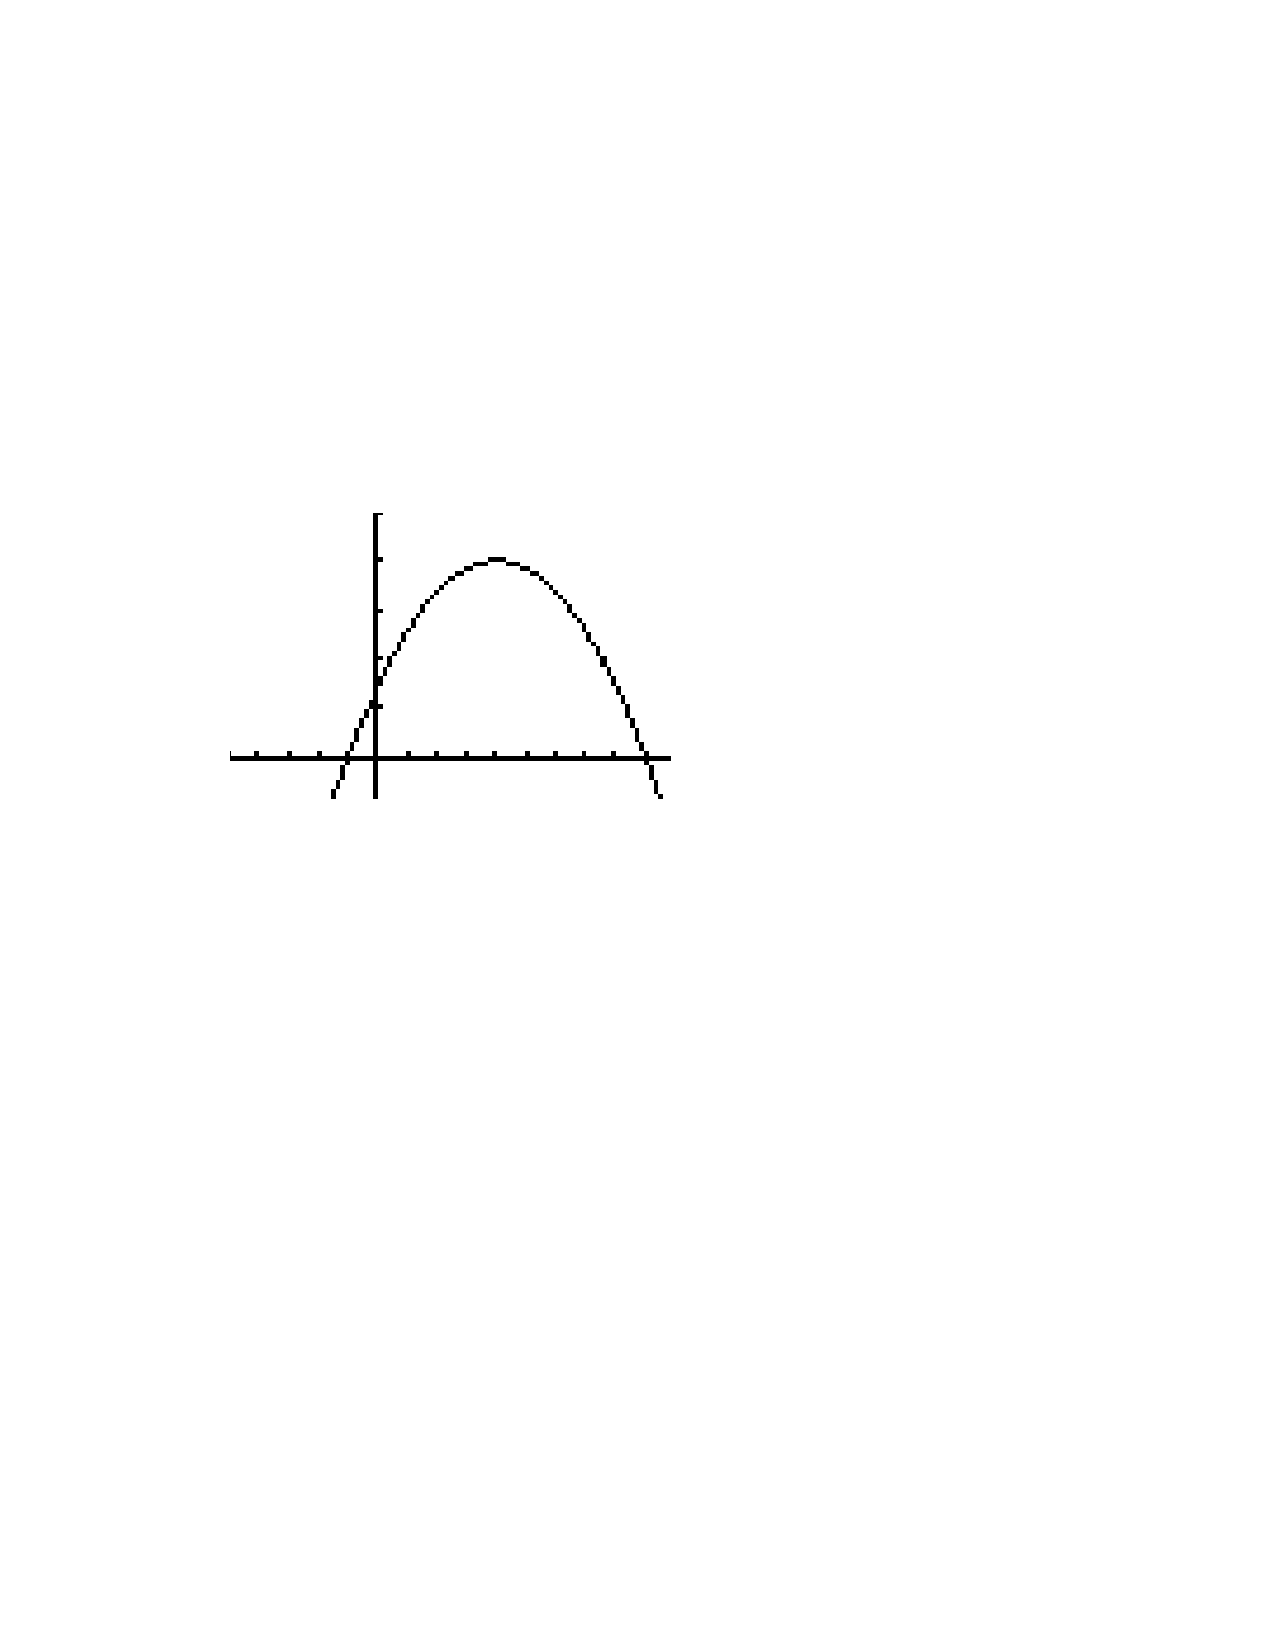
\includegraphics[trim= 170 420 250 180]{Figure1.pdf}
%\end{image}


\newcommand{\RR}{\mathbb R}
\renewcommand{\d}{\,d}
\newcommand{\dd}[2][]{\frac{d #1}{d #2}}
\renewcommand{\l}{\ell}
\newcommand{\ddx}{\frac{d}{dx}}
\newcommand{\dfn}{\textbf}
\newcommand{\eval}[1]{\bigg[ #1 \bigg]}

\usepackage{multicol}

\renewenvironment{freeResponse}{
\ifhandout\setbox0\vbox\bgroup\else
\begin{trivlist}\item[\hskip \labelsep\bfseries Solution:\hspace{2ex}]
\fi}
{\ifhandout\egroup\else
\end{trivlist}
\fi} %% we can turn off input when making a master document

\title{Recitation \#24 - 5.3 Fundamental Theorem of Calculus}  

\begin{document}
\begin{abstract}		\end{abstract}
\maketitle

\section*{Warm up:} 
True of False:  If $f$ is continuous on the closed interval $[a,b]$, then 
$$\ddx \left( \int_a^b f(t) \d t \right) = f(x)$$
		\begin{freeResponse}
		False.  $\ddx \left( \int_a^b f(t) \d t \right) = 0$ since $\int_a^b f(t) \d t$ is a constant and $\ddx (\text{constant}) = 0$.
		\end{freeResponse}	
		
		
		

	
	
	
	
	

\section*{Group work:}



%problem 1
\begin{problem}
Find the derivative of the following functions:
	\begin{multicols}{2}
	\begin{enumerate}
	
	%part a
	\item  $F(x) = \int_{\sqrt{x}}^1 \frac{t^2}{2 + 3t^4} \d t$
		\begin{freeResponse}
		First notice that
		$$ F(x) = \int_{\sqrt{x}}^1 \frac{t^2}{2 + 3t^4} \d t = - \int^{\sqrt{x}}_1 \frac{t^2}{2 + 3t^4} \d t .$$
		So we can apply the Fundamental Theorem of Calculus Part I, along with the chain rule, to compute:
			\begin{align*}
			F^\prime (x) &= \ddx \left( - \int^{\sqrt{x}}_1 \frac{t^2}{2 + 3t^4} \d t \right)  \\
			&= - \frac{(\sqrt{x})^2}{2 + 3(\sqrt{x})^4} \cdot \ddx(\sqrt{x})  \\
			&= - \frac{x}{2+3x^2} \cdot \frac{1}{2 \sqrt{x}}  \\
			&= - \frac{\sqrt{x}}{2(2+3x^2)}  
			\end{align*}
		\end{freeResponse}
		
		
		
	%part b
	\item  $G(x) = \int_x^{x^3} \sin(7t) \d t$
		\begin{freeResponse}
		First notice that
			\begin{align*}
			G(x) &= \int_x^{x^3} \sin(7t) \d t  \\
			&= \int_x^0 \sin(7t) \d t + \int_0^{x^3} \sin(7t) \d t  \\
			&=  - \int^x_0 \sin(7t) \d t + \int_0^{x^3} \sin(7t) \d t
			\end{align*}
		It is worth pointing out that breaking up the integral above at $0$ was arbitrary.  Since $\sin(7t)$ is continuous over $(-\infty, \infty)$, we could have chosen any real number in place of $0$.
		
		We can now apply the Fundamental Theorem of Calculus Part I, along with the chain rule, to compute:
			\begin{align*}
			G^\prime (x) &= \ddx \left( - \int^x_0 \sin(7t) \d t + \int_0^{x^3} \sin(7t) \d t \right)  \\
			&= \ddx \left( - \int^x_0 \sin(7t) \d t \right) + \ddx \left( \int_0^{x^3} \sin(7t) \d t \right)  \\
			&= -\sin(7x) + \sin(7x^3) \cdot \ddx(x^3)  \\
			&= 3x^2 \sin(7x^3) - \sin(7x)
			\end{align*}
		\end{freeResponse}
		
		
		
	\end{enumerate}
	\end{multicols}	
		
\end{problem}








\newpage







%problem 2
\begin{problem}
Given the following graph of $y=f(x)$, let $g(x) = \int_{-1}^x f(t) \d t$.
	\begin{enumerate}
	
	%part a
	\item  Is $g$ continuous?  Why or why not?
		%\begin{freeResponse}
		
		%\end{freeResponse}
		
		
		
	%part b
	\item  Is $g$ differentiable?  Why or why not?
		%\begin{freeResponse}
		
		%\end{freeResponse}
		
		
		
	%part c
	\item  Where does $g$ achieve its absolute maximum and minimum values?  Where does $g$ achieve any local extreme values?  Assume the domain of $g$ is $[-1,7.6]$.
		%\begin{freeResponse}
		
		%\end{freeResponse}
		
		
		
	%part d
	\item  Where is the graph of $g$ concave up?  Concave down?
		%\begin{freeResponse}
		
		%\end{freeResponse}
		
\begin{image}
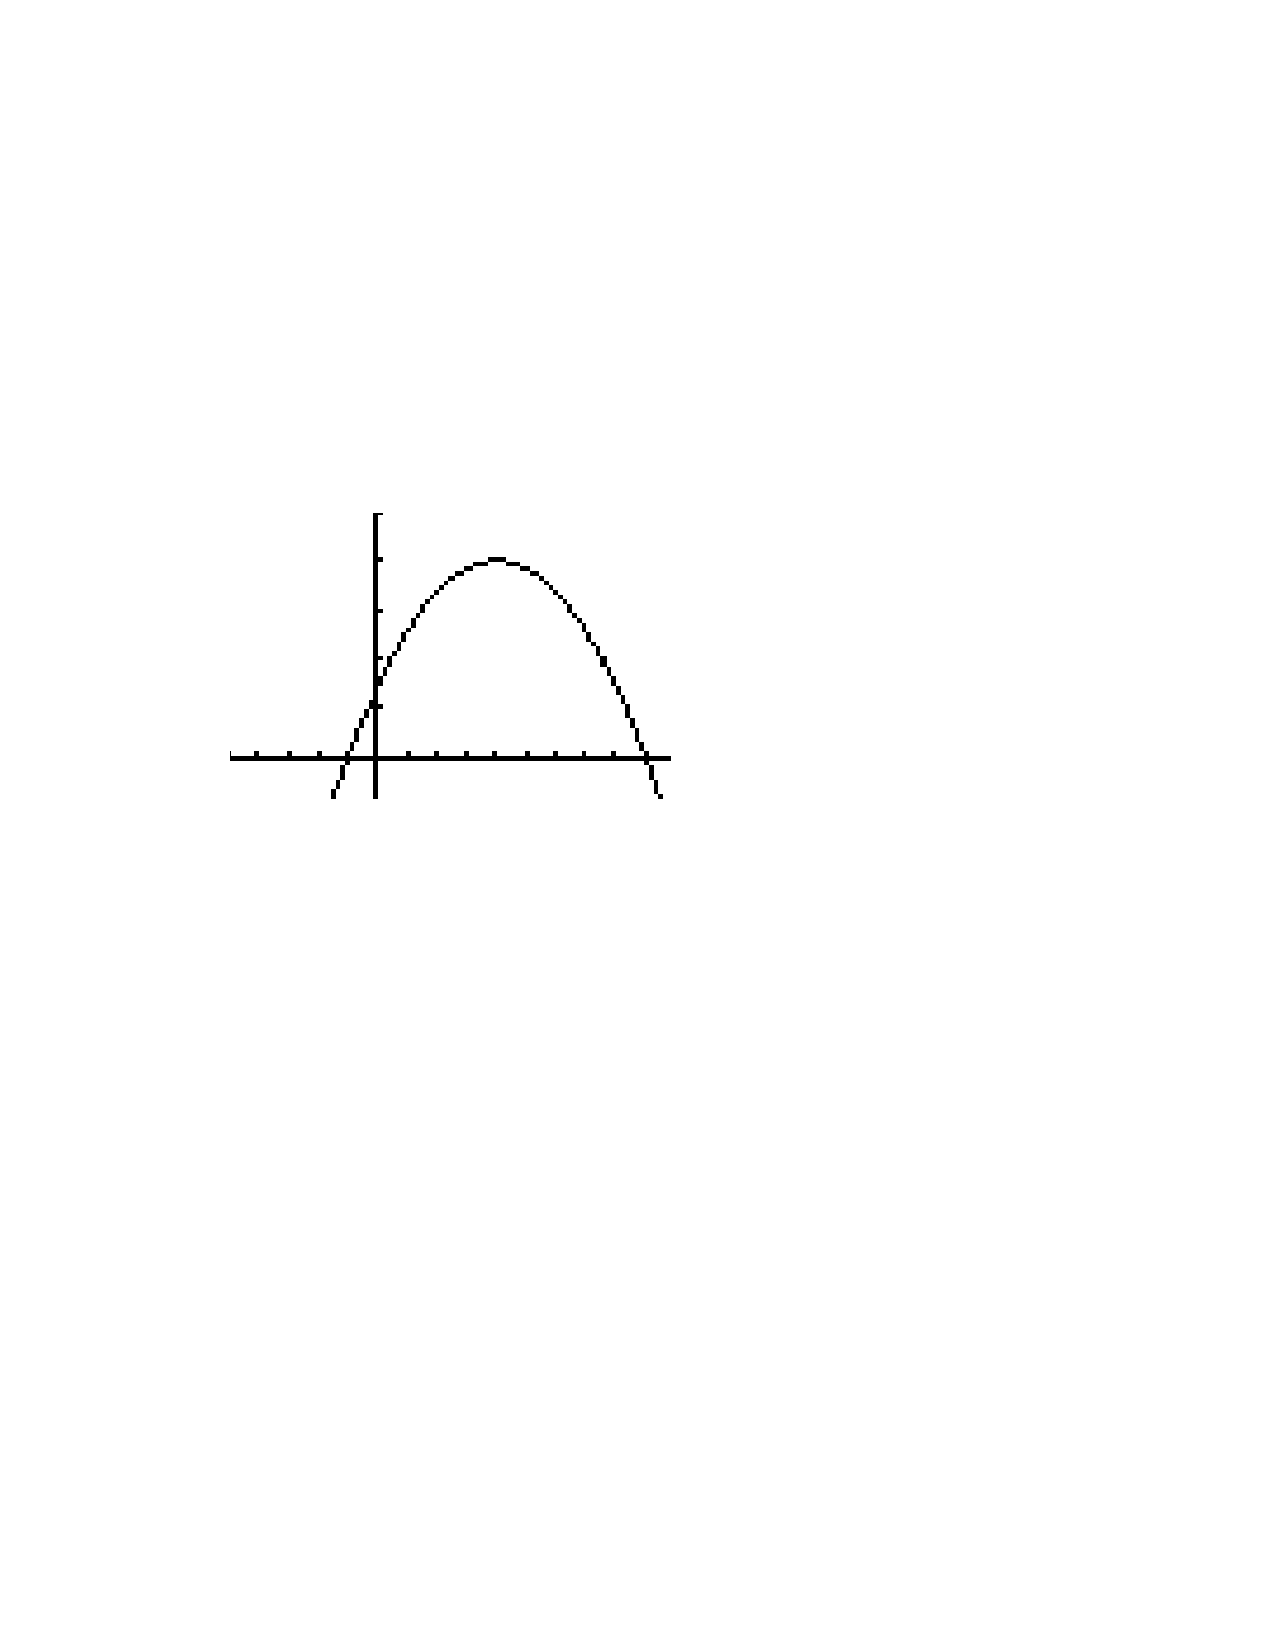
\includegraphics[trim= 100 440 250 170]{Figure1.pdf}
\end{image}

		\begin{freeResponse}
			\begin{enumerate}
			\item  $g(x)$ represents the area function (or the signed area between the curve$y=f(x)$ and the $x$-axis from -1 to $x$).  By the FTC(I), $g(x)$ is continuous.
			
			\item  Similarly by the FTC(I) the function $g$ is differentiable, and moreover:
			$$\ddx \left( g(x) \right) = \ddx \left( \int_{-1}^x f(t) \d t \right)= f(x)$$
			
			\item  Since $g$ is continuous on the closed interval $[-1,7.6]$, $g$ attains its absolute extreme values at either critical points or endpoints.  
			But we just saw that $g^\prime(x) = f(x)$, and so the critical points of $g$ are just the points where $f(x) = 0$.  
			Thus, the critical points of $g$ are approximately $3.1$ and $6.25$.
			
			Since $f = g^\prime$, $g$ is increasing when $f$ is positive and $g$ is decreasing when $f$ is negative.  
			So we have that $x=3.1$ is a local maximum while $x=6.25$ is a local minimum of $g$.  
			This takes care of the local extreme values.  
			
			To find the absolute extreme values of $g$, we need to reason out what are the largest and smallest values of $g(-1), g(3.1), g(6.25),$ and $g(7.6)$.  
			And do not forget the $g(x)$ denotes the (signed) area under the curve!  
			
			Clearly $g(-1) = 0$ since a line does not have any area.  
			At any time after $x=-1$ we have a positive (net) area.  
			Thus, our absolute minimum occurs at $x=-1$.
			To find the absolute maximum of $g$, we need to compare $x=3.1$ and $x=7.6$. 
			We see that we have the greatest area under the curve at $x=3.1$ because 
			by the time we get to $x=7.6$, the area we have subtracted off between $x=3.1$ and $x=6.25$ is greater than 
			what we have added back on from $x=6.25$ to $x=7.6$.  
			Therefore, our absolute maximum occurs at $x=3.1$.  
			
			
			\item  $g$ is concave up when $g''(x) = f'(x) > 0$.  But $f'(x) > 0$ when $f$ is increasing, which is on $(-1,0) \cup (4.25,7.6)$.  
			Similarly, $g$ is concave down when $f$ is decreasing, which is on $(0,4.25)$.  
			
			\end{enumerate}
		\end{freeResponse}
		
		
		
	\end{enumerate}

		
		
		

\end{problem}
	
	
	
	
	
	
	
	
			
			

%problem 3
\begin{problem}
Compute the following integrals:
	\begin{enumerate}
	
	%part a
	\item  $\int_0^1 e^{5x} \d x$
		\begin{freeResponse}
		$\int_0^1 e^{5x} \d x  = \eval{\frac{1}{5} e^{5x}}_0^1= \frac{1}{5} \left( e^5 - e^0 \right) = \frac{1}{5} (e^5 - 1)$
		\end{freeResponse}
		
		
		
	%part b
	\item  $\int\limits_{-2}^{-1} \frac{1}{x^3} \d x$
		\begin{freeResponse}
			\begin{align*}
			\int\limits_{-2}^{-1} \frac{1}{x^3} \d x &= \int\limits_{-2}^{-1} x^{-3} \d x  \\
			&= \eval{\frac{x^{-2}}{-2}}_{-2}^{-1}  \\
			&= \eval{\frac{-1}{2x^2}}_{-2}^{-1}  \\
			&= - \frac{1}{2} - \left( - \frac{1}{8} \right)  \\
			&= - \frac{1}{2} + \frac{1}{8} = - \frac{3}{8}
			\end{align*}
		\end{freeResponse}
		
		
		
	%part c
	\item  $\int _0^4 \left( 3x - 5 + 7 \sqrt{16-x^2} \right) \d x$
		\begin{freeResponse}
		First notice that:
		\begin{equation}\label{eq1}
		\int _0^4 \left( 3x - 5 + 7 \sqrt{16-x^2} \right) \d x = \int_0^4 ( 3x - 5) \d x + 7 \int_0^4 \sqrt{16-x^2} \d x.
		\end{equation}
		To get the easy part out of the way first:
		\begin{equation}\label{eq2}
		\int_0^4 (3x-5) \d x = \eval{\frac{3}{2} x^2 - 5x}_0^4 = (24 - 20) - (0-0) = 4. 
		\end{equation}
		So the real issue is in computing $\int_0^4 \sqrt{16-x^2} \d x$.  
		
		We do not know how to integrate $\sqrt{16-x^2}$ directly, but recall that the solution set to the equation $x^2 + y^2 = 16$ is a circle with radius $4$ centered at the origin.  
		Solving for $y$ we get $y = \pm \sqrt{16-x^2}$.  
		So if we restrict ourselves to $y=\sqrt{16-x^2}$ and $0 \leq x \leq 4$, this gives us the upper-right quarter of the circle (draw a picture and convince yourself of this).  
		Since the total area of the circle of $\pi (4)^2 = 16\pi$, the area under this portion of the curve is $\frac{1}{4} (16\pi) = 4\pi$.  
		Thus we have computed (geometrically) that 
		\begin{equation}\label{eq3}
		\int_0^4 \sqrt{16-x^2} \d x = 4\pi. 
		\end{equation}
		We can now finish the problem by plugging our solutions from equations \eqref{eq2} and \eqref{eq3} into equation \eqref{eq1}:
		$$\int _0^4 \left( 3x - 5 + 7 \sqrt{16-x^2} \right) \d x = 4 + 7(4\pi) = 4 + 28\pi. $$
		\end{freeResponse}
		
		
		
	\end{enumerate}

			
			
		
\end{problem}

















	
	
	
	
	
	
	
	
	

	










								
				
				
	














\end{document} 


















